\documentclass[
% twocolumn,
% hf,
]{ceurart}

%%
%% One can fix some overfulls
\sloppy

%%
%% Minted listings support 
%% Need pygment <http://pygments.org/> <http://pypi.python.org/pypi/Pygments>
%\usepackage{listings}
%% auto break lines
%\lstset{breaklines=true}

%\usepackage{cite}
\usepackage{amssymb,amsmath,amsthm,amsfonts}
\newtheorem{theorem}{Theorem}
\newtheorem{definition}{Definition}
\usepackage{mathtools} % Bonus
\usepackage{algorithmic}
\usepackage{graphicx}
\usepackage{textcomp}
\usepackage[dvipsnames]{xcolor}
\usepackage{url}
\usepackage{mathtools}
\usepackage{relsize}
\usepackage{tikz}
\usetikzlibrary{decorations.pathreplacing}
\usetikzlibrary{arrows.meta}

\usepackage[ruled,vlined]{algorithm2e}
\SetKwInOut{Input}{Input}
\SetKwInOut{Output}{Output}
\SetKwInOut{Ensures}{Ensures}
\SetKwInOut{Throws}{Throws}
\SetKw{Throw}{throw}
\SetKw{ThrowsKw}{throws}
\SetKw{Continue}{continue}
\SetKw{Var}{var}
\SetKw{Or}{or}
\SetKw{And}{and}
\SetKw{Not}{not}
\SetKw{record}{record}
\SetKwProg{function}{function}{}{end}
\SetKwProg{procedure}{procedure}{}{end}
\SetKwProg{thread}{thread}{}{end}
\SetKwProg{try}{try}{}{}
\SetKwProg{catch}{catch}{}{end}
\SetKwProg{forever}{forever}{}{end}
\SetKwProg{synchronized}{synchronized}{}{end}

\DeclareUrlCommand\email{\urlstyle{tt}}
\DeclareUrlCommand\website{\urlstyle{same}}
\DeclareUrlCommand\directory{\urlstyle{same}}
\newcommand{\hash}{{\mathit{hash}}}
\newcommand{\difficulty}{{\mathit{difficulty}}}
\newcommand{\delay}{{\mathit{delay}}}
\newcommand{\ie}{\emph{i.e.}\@}
\newcommand{\wrt}{\emph{wrt.}\@}
\newcommand{\Challenges}{{\mathsf{Challenges}}}
\newcommand{\generation}{{\mathit{generation}}}

\colorlet{lightred}{red!50!white}
\colorlet{verylightred}{red!20!white}
\colorlet{verylightyellow}{yellow!20!white}
\colorlet{verylightviolet}{violet!20!white}
\colorlet{verylightgreen}{green!20!white}
\colorlet{verylightgray}{gray!20!white}

\newcommand{\computer}{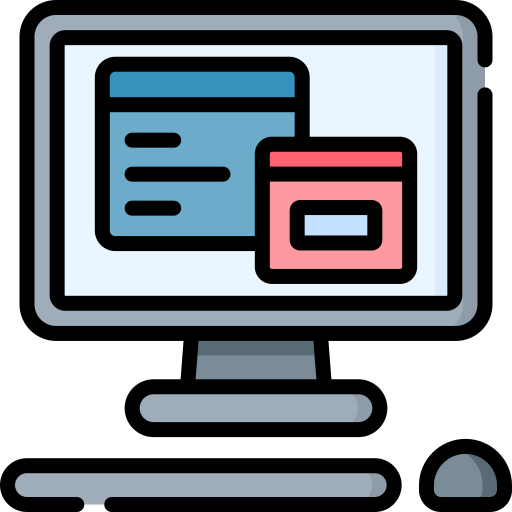
\includegraphics[width=1.3cm]{pictures/computer}}
\newcommand{\leftArrow}{
\includegraphics[width=0.6cm]{pictures/left_arrow}}
\newcommand{\signature}{
\includegraphics[width=0.3cm]{pictures/signature}}
\newcommand{\leftplug}{
\includegraphics[width=0.7cm]{pictures/plug_left}}
\newcommand{\rightplug}{
\includegraphics[width=0.7cm]{pictures/plug_right}}
\newcommand{\ssd}{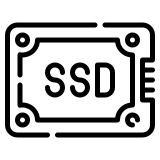
\includegraphics[width=0.8cm]{pictures/ssd}}
\newcommand{\numberofscoops}{{\#\mathit{scoops}}}
\newcommand{\scoop}{{\mathit{scoop}}}
\newcommand{\scoops}{{\mathit{scoops}}}
\newcommand{\scoopnumber}{{\mathit{scoopNumber}}}
\newcommand{\deadline}{{\mathit{deadline}}}
\newcommand{\Scoops}{{\mathsf{Scoops}}}
\newcommand{\Nonces}{{\mathsf{Nonces}}}
\newcommand{\nat}{\mathbb{N}}
\newcommand{\nonce}{{\mathit{nonce}}}
\newcommand{\Prologs}{{\mathsf{Prologs}}}
\newcommand{\private}{{\mathit{private}}}
\newcommand{\public}{{\mathit{public}}}
\newcommand{\chainid}{{\mathit{chainId}}}
\newcommand{\PrivateKeys}{{\mathsf{PrivateKeys}}}
\newcommand{\PublicKeys}{{\mathsf{PublicKeys}}}
\newcommand{\seed}{{\mathit{seed}}}
\newcommand{\finalhash}{{h_{\mathit{final}}}}
\newcommand{\Plots}{{\mathsf{Plots}}}
\newcommand*\xor{\oplus}
\newcommand{\nonces}{{\mathit{nonces}}}
\newcommand{\challenge}{{\mathit{challenge}}}
\newcommand{\beat}{{\mathit{beat}}}
\newcommand{\Deadlines}{{\mathsf{Deadlines}}}
\newcommand{\size}{{\mathit{size}}}
\newcommand{\waitingtime}{{\mathit{waitingTime}}}
\newcommand{\plot}{{\mathit{plot}}}
\newcommand{\key}{{\mathit{key}}}

\DeclareMathOperator*{\append}{\bowtie}

\begin{document}

\copyrightyear{2026}
\copyrightclause{Copyright for this paper by its authors.
  Use permitted under Creative Commons License Attribution 4.0
  International (CC BY 4.0).}

%%
%% This command is for the conference information
\conference{DLT'26: 8th Distributed Ledger Technology Workshop, June 04--06, 2026, Pula, Italy}

%%
%% The "title" command
\title{Mobile Mining for Proof of Space}
%\thanks{Thank funding institutions, if any.}

%%
%% The "author" command and its associated commands are used to define
%% the authors and their affiliations.
\author[1]{Fausto Spoto}[%
orcid=0000-0003-2973-0384,
email=fausto.spoto@univr.it
]
\cormark[1]
\fnmark[1]
\address[1]{Dipartimento di Informatica, Universit\`a di Verona, Verona, Italy}

\author[2]{Ana Lucia Zandomeneghi}[%
orcid=0000-0001-6140-8841,
email=ana.zandomeneghi@ufma.br
]
\fnmark[1]
\author[2]{Jos\'e Renato de Oliveira Lima}[%
orcid=0000-0001-7723-1454,
email=renato.jose@ufma.br
]
\fnmark[1]
\address[2]{Bacharelado Interdisciplinar em Ci\^encia e Tecnologia (BICT), UFMA, S\~ao Lu\'{\i}s do Maranh\~ao, Brazil}

\cortext[1]{Corresponding author.}
\fntext[1]{These authors contributed equally.}

\maketitle

\begin{abstract}
  This paper advocates the use of mobile devices for blockchain mining.
  They are a large and cheap hardware base, which is
  interesting to start up a new blockchain, when it is
  hard to convince people to install complex software
  on a continuously connected computer. Moreover, they allow mining in less fortunate
  countries, where powerful hardware is not available.
  This paper acknowledges that mainstream mobile devices
  have limitations that make most mining algorithms impractical,
  with the notable exception of proof of space. The latter preallocates
  large data on disk, later used for inexpensive mining,
  in terms of minimal CPU, RAM and data exchange costs: this
  copes with the constrained resources of the mobile device.
  This paper presents our new Android app Mokaminter for mining for blockchains based
  on the generic Mokamint proof of space engine.
  It experimentally confirms its low costs and reduced battery use.
  To the best of our knowledge,
  Mokaminter is the first mobile app for mining.
\end{abstract}

%%
%% Keywords. The author(s) should pick words that accurately describe
%% the work being presented. Separate the keywords with commas.
\begin{keywords}
  blockchain \sep
  proof of space \sep
  mining \sep
  mobile mining \sep
  energy consumption
\end{keywords}

\section{Introduction}\label{sec:introduction}

Blockchain is a distributed network of computers (\emph{peers}).
Each peer receives transaction requests, that eventually packs
into \emph{blocks}. These form a growing tree,
where each block points back to the previous one. Mining is the process of
block creation and includes a notion of chain quality to
decide which of the many tree branches emerges
as the best chain, on which all peers agree,
hence reaching \emph{consensus}. Mining
is often remunerated: block creators may
mint and earn some amount of cryptocurrency.

This abstract description is explicitly generic \wrt{}
the notion of transaction, irrelevant here: a transaction is an operation
that modifies the state of an abstract machine.
For instance, it is a money transfer in Bitcoin~\cite{Nakamoto08} or
the execution of some code over shared objects in Ethereum~\cite{AntonopoulosW25}.
This description is also generic \wrt{} the mining algorithm.
Bitcoin pioneered proof of work~\cite{DworkN92},
while more modern blockchains mostly use
proof of stake~\cite{Kwon14}, and this paper focuses on proof
of space~\cite{Spoto25}.
In Bitcoin's proof of work,
minted blocks carry evidence of the performance of some computational
work for their creation. The more this work, the higher the
likelihood for the blocks to be integrated in the best chain.
It is well-known that this induces high electricity costs for CPU
computation and data centers, with a high ecological impact (resource
consumption, e-waste). Moreover, this leads to the concentration of mining power
in countries where electricity is cheaper, against the idea of full decentralization.
Proof of stake emerged as a reaction to that. Its idea is that
only a restricted set of peers (\emph{validators}) create blocks.
This makes mining cheaper, efficient and ecologically sustainable.
Non-validators may stake on the success of validators. That introduces some
decentralization, but
proof of stake is generally considered as more centralized than proof of work.
Still, it is the most used mining algorithm.
The idea of proof of space~\cite{AbusalahACKPR17,AtenieseBFG14,CohenP19,DziembowskiFKP15,ParkKFGAP18,RenD16,Spoto25} is that blocks carry evidence
of the allocation of large data on disk, used for their creation.
The larger that data, the higher the likelihood that
blocks get included in the best chain. Proof of space is decentralized like
Bitcoin's proof of work and ecological like proof of stake.

This paper focuses on \emph{mobile mining}, that is,
on mining with a mainstream mobile device (typically, a phone or tablet).
In principle, this is appealing because:
%
\begin{itemize}
\item it leverages a huge existing hardware base, that otherwise remains unused
  for most of the time;
\item it introduces mining to a large portion of humanity, who owns a
  phone but not a powerful connected computer;
\item it can be easily updated, thanks to the automatic update system of mobile devices;
\item it simplifies the start-up of new blockchains, since it is easier to convince people
  to install an app than to run and maintain some software on an always connected computer.
\end{itemize}
%
Mobile mining has not been used yet because of the obvious limitations
of mobile devices \wrt{} battery capacity and network bandwidth, in particular
in least favorite countries.

This paper makes the following contributions:
%
\begin{enumerate}
\item it presents mobile mining, its power and limitations;
\item it shows how proof of space emerges as a niche solution, less sensitive
  to such limitations;
\item it presents Mokaminter, our actual Android app for mobile mining with proof of space;
\item it reports experiments with Mokaminter, discussing its minimal CPU, RAM and data exchange costs
  and its battery use, as well as the amount of crypto earned with different devices.
\end{enumerate}
%
Mokaminter is a miner for mobile devices, not a blockchain
peer: it does not hold nor exchange blocks, it does not host the blockchain,
it does not use a database: all that would be prohibitive on a mobile device.
Mokaminter connects and mines for an external peer that keeps the blockchain.

The rest of this paper is organized as follows.
Sec.~\ref{sec:related_work} discusses related work.
Sec.~\ref{sec:mining} gives a uniform description of various mining algorithms and
discusses if they can be used on a mobile device.
Sec.~\ref{sec:pos} describes Mokamint's proof of space mining algorithm.
Sec.~\ref{sec:mokaminter} describes the Mokaminter mobile app.
Sec.~\ref{sec:experiments} confirms its reduced costs with actual experiments.
Sec.~\ref{sec:conclusion} concludes.

\section{Related Work}\label{sec:related_work}

Proof of space is a mining algorithm where disk (currently SSD) space
is used instead of CPU power.
It is energetically more efficient than proof of work and
more decentralized than proof of stake.
A preliminary \emph{plotting phase}, that must be expensive, allocates large data on disk,
which is later used in a cheap
\emph{mining phase} to quickly answer
block creation challenges received from blockchain peers:
the probability of creating new blocks on top of the best chain
is proportional to the allocated data size.
Pioneering work~\cite{AtenieseBFG14,DziembowskiFKP15} introduced
formal proofs on persistent storage and showed that
on-demand recomputations (or \emph{replotting attacks}~\cite{BaigGP25}) are not viable,
due to high complexity pebbling graphs and Merkle trees:
any attempt to reduce the allocated space has a prohibitive recomputation cost.
A subsequent evolution~\cite{RenD16}
uses \emph{stacked expanders} to reduce the cost
and simplify proofs. The SpaceMint prototype~\cite{ParkKFGAP18},
now discontinued, showed the approach feasible and considered
mitigations to potential attacks, typical of
proof of space, such as mining on multiple chains and block/challenge grinding.
Chia~\cite{AbusalahACKPR17,CohenP19}, a more robust implementation, combines
space with verifiable delay functions, in a hybrid proof of space and time mechanism.
Filecoin~\cite{Fil24} lets parties commit space and prove, repeatedly,
that they still hold data in the committed space.
We build on the proof of space algorithm of Signum~\cite{signum}
based on the expensive precomputation of
plot files that later support cheap block creation, as formalized
in~\cite{Spoto25}. We work with peers built over the generic blockchain
engine Mokamint~\cite{mokamint-source-code},
derived from Signum's algorithm, but generic \wrt{} the
notion of transactions, delegated to an application layer.

There is a lack of scientific research on the use of mobile devices
for blockchain mining.
In~\cite{LeePSB20}, a system is proposed to build local
industrial IoT blockchains, where drones are mobile miners
with proof of work. It does not scale
to a global blockchain and to mainstream mobile devices, that
are not competitive against expensive specialized hardware and whose limited battery
cannot sustain the proof of work.
The same limitation applies to~\cite{SuankaewmaneeHN18}, that
presents a specialized blockchain for mobile commerce, with Android phones as
mobile miners with proof of work.
Experiments are reported for blocks holding up to six transactions, which is
sensible for a local blockchain but irrealistic for a global one.
Despite its title, \cite{JiangLW22}~tackles another problem, namely,
offloading blockchain applications
to a cloud computing provider to make them usable
with the limited resources of a phone.
More generally, this allows edge devices, with strong hardware limitations,
to offload expensive computations
to external servers and to the cloud~\cite{SoundararajS25}.
The goal of the present paper is instead to perform mining \emph{in} the mobile device
and let blockchain peers leverage many
mainstream mobile devices running a mining app.

A simple search on Google Play reports a few Android apps for
\emph{crypto mining}. Despite their name, these apps are not miners, but either
mobile dashboards to cloud pool miners (mining occurs in the cloud and
the app is just monitoring, see for instance~\cite{ctpool-google-play,viabtc-google-play,ecos-google-play,cloudminingbitcoincrypto-google-play,minex-google-play}),
or dubious games that promise Bitcoins in exchange of solving tasks
or watching ads (such as~\cite{bitcoinminerearnrealcrypto-google-play,cryptofortunetycoonbtcminer-google-play}).
In particular, our research did not find any app for actually mining \emph{in}
a mainstream mobile device.

\section{An Abstract Presentation of Mining}\label{sec:mining}

Different mining algorithms fit
inside the uniform setting of a competitive game
played, concurrently and independently, by the peers of a blockchain network, whose
goal is to decide which peer may add a \emph{valid} \textbf{next}
block to the stable chain. \emph{Valid} means that it respects
all consensus rules. For instance,
it points back to an existing block and
includes transactions with valid signatures
(the full, large list of consensus rules is outside the topic of this paper).
The game works in terms of:
%
\begin{itemize}
\item \emph{challenge}: from the current chain $\xi$,
  compute, deterministically, a challenge for \textbf{next};
\item \emph{answer}: create, if possible,
  a \textbf{next} that satisfies the challenge;
\item \emph{competition}: among more possible \textbf{next}s, prefer the \emph{best}
  one \wrt{} some notion of chain quality.
\end{itemize}
%
Each peer runs this mining algorithm,
whispers its resulting \textbf{next} to its
connected peers and receives the \textbf{next} of its connected peers. In case
of more alternative \textbf{next}s, the competition rule lets one choose the
winner. This gives rise to a \emph{consensus algorithm} that uses the mining
algorithm as a subroutine.

For proof of work, the mining game becomes:
%
\begin{itemize}
\item \emph{challenge}: compute an integer $\difficulty$ from $\xi$
  and find a valid \textbf{next} such that $\hash(\mathbf{next})\ge\difficulty$;
\item \emph{answer}: create a \textbf{next} by rotating the possible
  values for its nonce field, until $\hash(\mathbf{next})\ge\difficulty$;
\item \emph{competition}: among more \textbf{next}s, prefer that with the largest hash.
\end{itemize}
%
The computation of $\difficulty$ is not relevant here.
Moreover, Bitcoin's proof of work is usually given
in terms of a \emph{smallest} hash, but we require (equivalently) the
\emph{largest} hash to match the intuition that a higher $\difficulty$ makes mining harder.

For proof of stake, it is generally accepted that there is
\emph{no} mining~\cite{Kwon14}, but a mining game can be defined also in this case:
%
\begin{itemize}
\item \emph{challenge}: compute an integer $i$ from $\xi$ (the index of the chosen
  validator);
\item \emph{answer}: the $i$th validator
  creates a valid \textbf{next}; the others do not create anything and
  wait to receive \textbf{next};
\item \emph{competition}: among more possible \textbf{next}s, choose any of them, since
  this should not occur for this mining algorithm.
\end{itemize}
%
The algorithm for computing $i$ is irrelevat here: often, it is a simple
round-robin. Moreover, the consensus algorithm typically enriches the above
mining algorithm with a Byzantine protocol of pre-votes and pre-commits~\cite{Kwon14}.

Finally, proof of space, as presented in~\cite{Spoto25},
is based on the idea that \textbf{next} must contain
a data structure, called \emph{nonce}, that can be quickly recovered from a
set of precomputed nonces on disk (the \emph{plot file}). The mining game in this case is:
%
\begin{itemize}
\item \emph{challenge}: compute some data $\kappa$ from $\xi$;
\item \emph{answer}: create a valid \textbf{next} block, containing a nonce $\nu$
  derived from the plot file and from $\kappa$;
\item \emph{competition}: among more possible \textbf{next}s, choose that with the smallest
  $\delay(\nu,\kappa)$, where $\nu$ is the nonce in \textbf{next}.
\end{itemize}
%
The challenge $\kappa$ is used to select a nonce, from the plot file, that minimizes
$\delay$. The key point of this mining algorithm
is that the computation of the nonces (\ie{}, of the plot file) is so expensive
that it cannot be done on-the-fly, for each mined block, but rather
once and for all, before starting mining. The plot remains on disk to answer, quickly, mining
challenges. The consensus algorithm uses $\delay$ to wait until the block becomes valid.

This abstract presentation of mining clarifies
that mining is a subroutine whose input is the challenge derived from the current
chain $\xi$ and whose output is the answer \ie{}, the information
needed to create \textbf{next}:
a nonce for proof of work and proof of space (although a different notion of nonce is
used in either case), and a Boolean for proof of stake
(create the block or rather let another validator do it).
Fig.~\ref{fig:mining} shows this:
the miner that provides the answer to create \textbf{next}
and the peer that actually creates \textbf{next}
are separate software parts of the same tool. Traditionally,
such software parts work in the same machine.
But they have been already moved to different machine, for instance in pool
mining architectures, where a single peer leverages the power of many, remote
miners, working in different machines and connected through a network
(Fig.~\ref{fig:mining}).
Namely, many users want to run a miner and earn cryptos,
but only a few are interested in running a full blockchain peer on a dedicated machine,
which requires technical skills, database space and a very good internet connection.

\begin{figure}[t]
  \begin{center}
    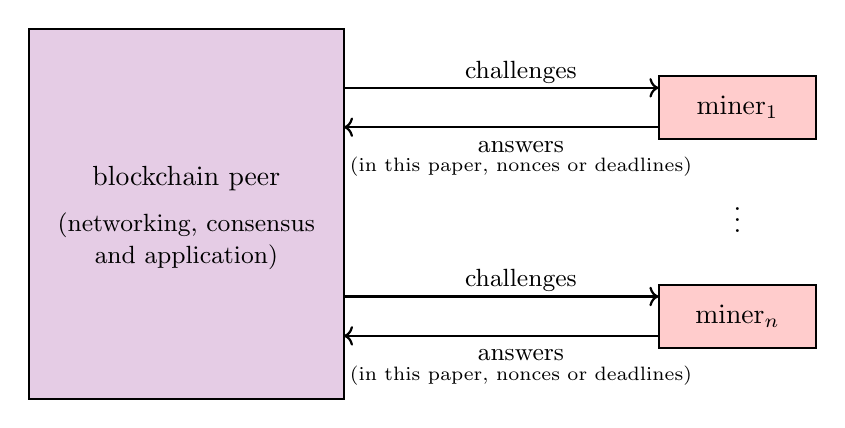
\begin{tikzpicture}
      \draw [fill=verylightviolet,thick] (-1,-0.3) rectangle +(4,4.7);
      \draw (1,2.5) node {blockchain peer};
      \draw (1,1.9) node {{\small (networking, consensus}};
      \draw (1,1.5) node {{\small and application)}};

      \draw [fill=verylightred,thick] (7,3) rectangle +(2,0.8);
      \draw (8.0,3.4) node {$\text{miner}_1$};
      \draw[->, thick] (3,3.65) -- (7,3.65);
      \draw (5.25,3.85) node {{\small challenges}};
      \draw[<-, thick] (3,3.15) -- (7,3.15);
      \draw (5.25,2.9) node {{\small answers}};
      \draw (5.25,2.65) node {{\scriptsize (in this paper, nonces or deadlines)}};

      \draw (8.0,2.075) node {$\vdots$};

      \draw [fill=verylightred,thick] (7,0.35) rectangle +(2,0.8);
      \draw (8.0,0.75) node {$\text{miner}_n$};
      \draw[->, thick] (3,1.0) -- (7,1.0);
      \draw (5.25,1.2) node {{\small challenges}};
      \draw[<-, thick] (3,0.5) -- (7,0.5);
      \draw (5.25,0.25) node {{\small answers}};
      \draw (5.25,0) node {{\scriptsize (in this paper, nonces or deadlines)}};
    \end{tikzpicture}
  \end{center}
  \caption{Blockchain peer and miner(s) as separate software tools, possibly
    running in different machines connected through a network.}\label{fig:mining}
\end{figure}

Up to now, the machines where the miners are running
are computers or specialized, very expensive hardware. The goal of this article
is to allow such miners to run inside a mobile device as well.
But this might result impossible or impractical,
depending on the mining algorithm and on the machine
where the miner will run. Let us consider, in particular, the case when
the mining algorithm is one of those discussed
in Sec.~\ref{sec:introduction}.

\subsubsection*{Proof of work}
%
In this case, the challenge includes the full block being
created, since its nonce must maximize its hash.
For Bitcoin, a block's size is up to 4~MB after the Segregated Witness upgrade.
This data must be exchanged at \emph{each} block creation, impossible in many
countries where mobile internet is slow; moreover, most mobile operators limit
the exchanged GB per month; finally, the computational cost
of proof of work would drain the battery of the mobile device. Consequently,
at the moment, mining with proof of work is irrealistic on a mobile device,
for a global blockchain such as Bitcoin.

\subsubsection*{Proof of stake}
%
In this case, mining is very cheap and limited to the validators. The exchanged data is minimal.
But validators have no reason to offload their very simple mining activity.
Therefore, mining on a mobile device is possible for proof of stake, but it does
not seem of any practical interest.

\subsubsection*{Proof of space}
%
In this last case, mining requires the use of disk space, but no significant
CPU power. Currently, mobile devices have an average disk space
of 256~GB, smaller than the average 1000~GB of desktop computers but still significant.
Moreover, the proof of space of~\cite{Spoto25} uses very small challenges (around 64~bytes)
and answers (nonces, compacted into \emph{deadlines} of around 200~bytes).
The block being created is not needed for mining. This makes that
algorithm ideal for a remote miner in a mobile device:
no need of significant CPU power, enough disk space in the device and little data exchange.
This is why it has been the choice for the implementation of our Mokaminter app.

\section{Mokamint's Proof of Space Mining Algorithm}\label{sec:pos}

Mokamint uses a mining algorithm based on a specific instance of proof of space,
derived from Signum's. The idea is relatively simple: each peer
allocates, on disk, its own \emph{plot}, \ie{}, a set of data structures called \emph{nonces}.
A nonce (Fig.~\ref{fig:waiting_time_nonce}) is an array of bytes, split into chunks called \emph{scoops}.
Whenever a peer needs to create a new block, to expand a chain of blocks $\xi$,
it computes a \emph{challenge} from $\xi$ that sends to its miner (Fig.~\ref{fig:mining}). The miner uses
that challenge to compute the minimal waiting time among that of the nonces
in its plot on disk (Fig.~\ref{fig:waiting_time_plot}).
The nonce that generates the minimal
waiting time is sent to the peer, that will selevct the minimal waiting time among those
of all its connected miners and use it to build the block that expands $\xi$.
That block can then be propagated to all peers, but only after the waiting time has elapsed,
or otherwise other peers might reject it as (still) invalid.

\begin{figure}[t]
  \begin{center}
    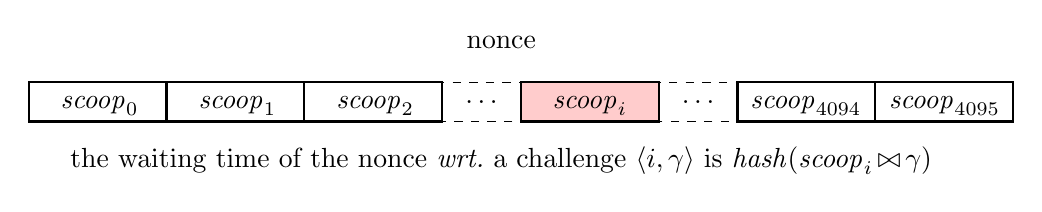
\begin{tikzpicture}[scale=1]

      \draw (-5.5,1) node {nonce};
      \draw [thick] (-11.5,0) rectangle +(1.75,0.5);
      \draw (-10.6,0.2) node {$\scoop_0$};
      \draw [thick] (-9.75,0) rectangle +(1.75,0.5);
      \draw (-8.85,0.2) node {$\scoop_1$};
      \draw [thick] (-8,0) rectangle +(1.75,0.5);
      \draw (-7.1,0.2) node {$\scoop_2$};
      \draw [dashed] (-6.25,0) rectangle +(1,0.5);
      \draw (-5.75,0.25) node {$\ldots$};
      \draw [thick,fill=verylightred] (-5.25,0) rectangle +(1.75,0.5);
      \draw (-4.375,0.2) node {$\scoop_i$};
      \draw [dashed] (-3.5,0) rectangle +(1,0.5);
      \draw (-3,0.25) node {$\ldots$};
      \draw [thick] (-2.5,0) rectangle +(1.75,0.5);
      \draw (-1.63,0.2) node {$\scoop_{4094}$};
      \draw [thick] (-0.75,0) rectangle +(1.75,0.5);
      \draw (0.13,0.2) node {$\scoop_{4095}$};

      \draw (-5.5,-0.5) node {the waiting time of the nonce \wrt{} a challenge $\langle i,\gamma\rangle$ is $\hash(\scoop_i\append\gamma)$};
%      \draw (-5.5, -0.9) node {normalized \wrt{} the current acceleration of the network};

    \end{tikzpicture}
  \end{center}
  \caption{A nonce is an array of bytes, split into chunks called scoops.
    The computation of the waiting time of a nonce \wrt{} the challenge
    $\langle i,\gamma\rangle$ selects the $i$th scoop of the nonce
    and computes a hash value that is interpreted as a numerical waiting time.}\label{fig:waiting_time_nonce}
\end{figure}

Let us formalize these mining algorithm now.
%
\begin{definition}[Challenge]\label{def:challenge}
  The set of \emph{challenges} is
  \[
  \Challenges=\left\{\langle\scoopnumber,\gamma\rangle\left|
  \begin{array}{l}
    0\le\scoopnumber<4096\text{ and $\gamma$ is a hash}
  \end{array}
  \right.\right\}.
  \]
  The $\gamma$ component of a challenge is said to be its \emph{generation}.
\end{definition}
%
The intuition is that $\gamma$ is a sort of digest of the history of the chain $\xi$ that
one wants to expand with a next block. Sec.~\ref{sec:blockchain_construction} will
show how a challenge is derived from $\xi$.

A \emph{scoop} is a pair of hashes. A \emph{nonce} is a \emph{progressive number} $p$, and
a list of $4096$ scoops (see Fig.~\ref{fig:waiting_time_nonce}, where the progressive
number is not shown, for simplicity).
%
\begin{definition}[Scoop, Nonce]\label{def:scoop_nonce}
  The sets of \emph{scoops} and \emph{nonces} are
  \begin{align*}
    \Scoops&=\left\{\langle h_1,h_2\rangle\left|\begin{array}{l}
    h_1,h_2\text{ are hashes}
    \end{array}\right.\right\},\\
    \Nonces&=\left\{\langle p,\scoops\rangle\left|\begin{array}{l}
    p\in\nat\text{ and }\scoops\in\Scoops^{4096}
    \end{array}\right.\right\}.
  \end{align*}
\end{definition}

\begin{figure}[t]
  \begin{center}
    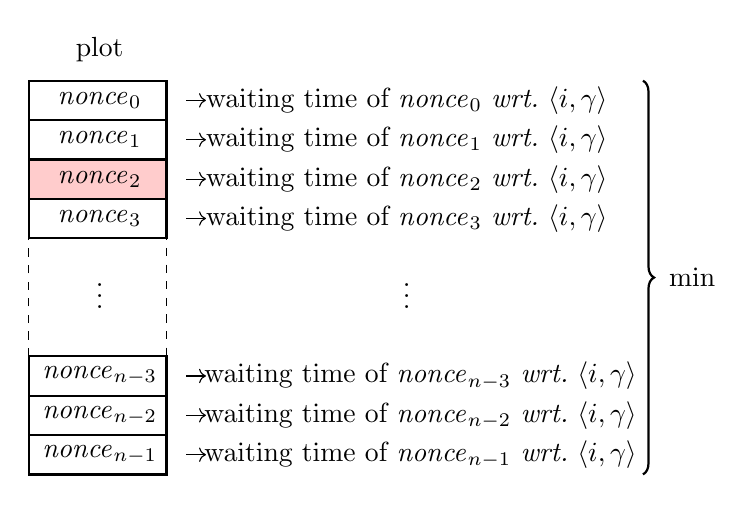
\begin{tikzpicture}[scale=1]

      \draw (0.4,5.4) node {plot};

      \draw [thick] (-0.5,4.5) rectangle +(1.75,0.5);
      \draw (0.4,4.75) node {$\nonce_0$};
      \draw[->] (1.5,4.75) -- +(0.25,0);
      \draw (4.3,4.75) node {waiting time of $\nonce_0$ \wrt{} $\langle i,\gamma\rangle$};

      \draw [thick] (-0.5,4) rectangle +(1.75,0.5);
      \draw (0.4,4.25) node {$\nonce_1$};
      \draw[->] (1.5,4.25) -- +(0.25,0);
      \draw (4.3,4.25) node {waiting time of $\nonce_1$ \wrt{} $\langle i,\gamma\rangle$};

      \draw [thick,fill=verylightred] (-0.5,3.5) rectangle +(1.75,0.5);
      \draw (0.4,3.75) node {$\nonce_2$};
      \draw[->] (1.5,3.75) -- +(0.25,0);
      \draw (4.3,3.75) node {waiting time of $\nonce_2$ \wrt{} $\langle i,\gamma\rangle$};

      \draw [thick] (-0.5,3) rectangle +(1.75,0.5);
      \draw (0.4,3.25) node {$\nonce_3$};
      \draw[->] (1.5,3.25) -- +(0.25,0);
      \draw (4.3,3.25) node {waiting time of $\nonce_3$ \wrt{} $\langle i,\gamma\rangle$};

      \draw (0.4,2.375) node {$\vdots$};
      \draw [dashed] (-0.5,1.5) rectangle +(1.75,1.5);
      \draw (4.3,2.375) node {$\vdots$};

      \draw [thick] (-0.5,1) rectangle +(1.75,0.5);
      \draw (0.4,1.25) node {$\nonce_{n-3}$};
      \draw[->] (1.5,1.25) -- +(0.25,0);
      \draw (4.475,1.25) node {waiting time of $\nonce_{n-3}$ \wrt{} $\langle i,\gamma\rangle$};

      \draw [thick] (-0.5,0.5) rectangle +(1.75,0.5);
      \draw (0.4,0.75) node {$\nonce_{n-2}$};
      \draw[->] (1.5,0.75) -- +(0.25,0);
      \draw (4.475,0.75) node {waiting time of $\nonce_{n-2}$ \wrt{} $\langle i,\gamma\rangle$};

      \draw [thick] (-0.5,0) rectangle +(1.75,0.5);
      \draw (0.4,0.25) node {$\nonce_{n-1}$};
      \draw[->] (1.5,0.25) -- +(0.25,0);
      \draw (4.475,0.25) node {waiting time of $\nonce_{n-1}$ \wrt{} $\langle i,\gamma\rangle$};

      \draw [decorate,decoration={brace,amplitude=4pt},thick,xshift=0.1cm,yshift=0pt]
      (7.2,5) -- (7.2,0) node [midway,right,xshift=.2cm] {$\min$};

    \end{tikzpicture}
  \end{center}
  \caption{A plot is a set of nonces. Its waiting time
    \wrt{} a challenge $\langle i,\gamma\rangle$ is the minimal waiting time among those of its nonces
    \wrt{} $\langle i,\gamma\rangle$ (Fig.~\ref{fig:waiting_time_nonce}).
    For instance, it might be that of $\nonce_2$ in the picture.}\label{fig:waiting_time_plot}
\end{figure}

A \emph{prolog} identifies the parts involved in mining: the peer, the miner (Fig.~\ref{fig:genericity})
and the chain identifier of the blockchain for which mining is performed.
%
\begin{definition}[Prolog]\label{def:prolog}
  The set of \emph{prologs} is
  \[
  \Prologs=\left\{\langle\mathit{key}_\public^{\mathit{peer}},
  \mathit{key}_\public^{\mathit{miner}},\chainid\rangle\left|\begin{array}{l}
  \text{where $\mathit{key}_\public^{\mathit{peer}}$
    and $\mathit{key}_\public^{\mathit{miner}}$ are the public keys}\\
  \text{that identify a peer and a miner, respectively,}\\
  \text{and $\chainid$ is the chain identifier of a blockchain}
  \end{array}\right.\right\}.
  \]
\end{definition}
%
Prologs are relevant since they are used to mark nonces:
each nonce and consequently each plot is \emph{for a given prolog}.
Therefore, a miner cannot use the same plot for mining for more peers or for more
chains.

Def.~\ref{def:nonce_construction} formalizes the construction of a nonce, given its progressive number and a prolog. It uses a constant $\kappa>0$
to limit its computational cost, by avoiding hashing very large chunks of data.
The construction algorithm derives a sequence of hashes (steps~\ref{step:nonce_construction:seed}
and~\ref{step:nonce_construction:first_hash}) and constructs a \emph{final} hash from
all of them (step~\ref{step:nonce_construction:final_hash}) that uses to modify
the original sequence of hashes (step~\ref{step:nonce_construction:modify}).
Then it shuffles the sequence (step~\ref{step:nonce_construction:swap}), which intuitively
guarantees that, in order to compute a given scoop of the nonce
(\ie{}, a pair of consecutive hashes), the algorithm must be thoroughly executed.
%
\begin{definition}[$\nonce(p,\pi)$]\label{def:nonce_construction}
  Given $p\in\mathbb{N}$ and $\pi\in\Prologs$, let
  \[
  \nonce(p,\pi)=\langle p,\langle h_0,h_1\rangle\append
  \cdots\append\langle h_{2\cdot 4096-2},h_{2\cdot 4096-1}\rangle\rangle\in\Nonces,
  \]
  where the hashes $h_0,\ldots,h_{2\cdot 4096-1}$ are constructed as follows:
  %
  \begin{enumerate}
  \item\label{step:nonce_construction:seed} let $\seed=\pi.\mathit{key}^{\mathit{peer}}_{\public}\append
    \pi.\mathit{key}^{\mathit{miner}}_{\public}\append\pi.\mathit{chainid}\append p$;
  \item\label{step:nonce_construction:first_hash}
    for each $i$ from $2\cdot 4096-1$ to $0$, let
    \[
    h_i=\hash\left(\text{first $\kappa$ bytes of}\left(\left(\append_{i<j<2\cdot 4096}h_j\right)\append\seed\right)\right);
    \]
  \item\label{step:nonce_construction:final_hash}
    let
    $
    \finalhash=\hash\left(\left(\append_{0\le j<2\cdot 4096}h_j\right)\append\seed\right);
    $
  \item\label{step:nonce_construction:modify} for each $i$ from $0$ to $2\cdot 4096-1$, reassign
    $h_i$ to $h_i\xor\finalhash$;
  \item\label{step:nonce_construction:swap}
    for each odd $i$ from $1$ to $2\cdot 4096-1$, swap
    $h_i$ with $h_{2\cdot 4096-i}$.
  \end{enumerate}
\end{definition}
%
Let us discuss Def.~\ref{def:nonce_construction} now.
Step~\ref{step:nonce_construction:seed} starts a chain of hash computations that includes the prolog $\pi$
in the seed. As a consequence, the resulting nonces will be \emph{for $\pi$}: for instance,
the nonces of another peer or of another miner or for another chain identifier
will have a different $\pi$ and consequently
they will be different nonces.
Step~\ref{step:nonce_construction:first_hash} is a loop that computes all $h_i$ from the seed.
It uses a hashing function $\hash$ that is expected to be expensive to compute, such
as shabal256: this makes it hard to recompute nonces and plots on-the-fly (which would
be a proof of work algorithm) rather than once and for all before mining.
Step~\ref{step:nonce_construction:final_hash} computes a digest $\finalhash$ of all $h_i$'s and
step~\ref{step:nonce_construction:modify} uses that digest to make each $h_i$ dependent on all others, so that
one must compute them all in order to compute each of them.
This is strengthened by the traditional use of $\oplus$ (the bitwise xor function) to minimize the information loss.
Step~\ref{step:nonce_construction:swap} makes each scoop include a $h_i$ with $i\ge 4096$,
so that smaller scoops are not easier to compute than the others. This avoids a potential
time/memory tradeoff attack~\cite{ParkKFGAP18}.

Mokamint miners hold one or more plots on disk. Their initialization is performed
only once and offline, hence it is not part of the mining protocol.
Namely, a plot is a set of nonces constructed according to Def.~\ref{def:nonce_construction},
for a finite non-empty set of progressive numbers $P$ and
for a given prolog $\pi$.
%
\begin{definition}[Plot]\label{def:plot}
  The set of \emph{plots} is defined as
  \[
  \Plots=\left\{\left<\pi,\nonces\right>\left|\begin{array}{l}
  \pi\in\Prologs,\ \varnothing\not=P\subset\mathbb{N}\text{ is finite and }
  \nonces=\left\{\nonce(p,\pi)\left|\;p\in P\right.\right\}
  \end{array}\right.\right\}.
  \]
\end{definition}

Given a challenge and a nonce, the latter has a \emph{waiting time} that specifies how well
the nonce answers the challenge (Fig.~\ref{fig:waiting_time_nonce}).
%
\begin{definition}[$\mathit{waitingTime}(\nonce,\challenge)$]\label{def:nonce_value}
  Let $\nonce\in\Nonces$ and $\challenge\in\Challenges$.
  The \emph{waiting time of $\nonce$ \wrt{} $\challenge$} is
  \[
    \mathit{waitingTime}(\nonce,\challenge)=\hash(\nonce.\scoops[\challenge.i]\append\challenge.\gamma).
  \]
\end{definition}
%
Miners use the waiting time of their nonces
to choose the best nonce for each given challenge,
\ie{}, the one with minimal value (Fig.~\ref{fig:waiting_time_plot}).
Note that only the $(\challenge.i)\mathit{th}$ scoop is used to compute that value.
That is, Mokamint consults only a small portion of the whole plot
file at each mining challenge.
That nonce could then be sent to the peer as answer for
the challenge (Fig.~\ref{fig:mining}).
But nonces are relatively big: around $262$ kbytes. Since they
must be stored in blockchain, inside each block, and since they should be
exchanged between miner and peer
(Fig.~\ref{fig:mining}), a more compact data structure is needed.
\emph{Deadlines} are exactly this compact data structure
that represents the nonce computed for a challenge.
Namely, a deadline carries the information needed
to reconstruct the nonce (progressive $p$ and prolog $\pi$, see Def.~\ref{def:nonce_construction}),
the value of that nonce (to avoid its repeated expensive recomputation through the formula
in Def.~\ref{def:nonce_value}), and
the challenge that that nonce was meant to answer. Therefore, in Fig.~\ref{fig:genericity}, the miner
will actually send back deadlines rather than nonces to the peer, which reduces the
data throughput. This is paramount if peer and miner are connected through a network rather
than being in the same physical machine.
%
\begin{definition}[Deadline]\label{def:deadline}
  The set of \emph{deadlines} is
  \[
  \Deadlines=\left\{
  \langle p,\pi,\mathit{value},\challenge\rangle
  \left|\begin{array}{l}
  \pi\in\Prologs,\ p\in\mathbb{N},\ \mathit{value}\text{ is a hash}\\
  \text{and }\challenge\in\Challenges
  \end{array}
  \right.
  \right\}.
  \]
\end{definition}
%
When a miner has selected its best nonce for a challenge, from a plot with prolog $\pi$,
and wants to send it to the peer,
it actually sends the much smaller deadline $\delta(\nonce,\pi,\challenge)$.
%
\begin{definition}[$\delta(\nonce,\pi,\challenge)$]\label{def:deadline_from_nonce}
  Given $\nonce\in\Nonces$, $\pi\in\Prologs$ and $\challenge\in\Challenges$, the
  \emph{deadline computed from $\nonce$ for $\pi$ and $\challenge$} is
  $\delta(\nonce,\pi,\challenge)=\langle\nonce.p,\pi,\mathit{value}(\nonce,\challenge),\challenge\rangle$.
\end{definition}

\begin{algorithm}[t]
  \Input{a $\plot$, already computed on disk}
  \Input{the peer $P$ connected to $M$}
  \BlankLine
  \thread{$\mathsf{mineDeadline}(\plot,P)$}{
    \forever{}{
      \nl\label{step:deadline_mining:wait}
      wait to receive a $\challenge\in\Challenges$ from $P$\;
      %
      \nl\label{step:deadline_mining:minimize}
      identify the $\nonce\in\plot.\nonces$ that minimizes its waiting time
      \wrt{} $\challenge$ (Def.~\ref{def:nonce_value})\;
      %
      \nl\label{step:deadline_mining:compute_deadline}
      send $\delta(\nonce,\plot.\pi,\challenge)$ to $P$ (Def.~\ref{def:deadline_from_nonce})\;
    }
  }
  \caption{The deadline mining algorithm, performed by each miner $M$ in its own thread.}
  \label{alg:deadline_mining}
\end{algorithm}

Alg.~\ref{alg:deadline_mining} is executed, inside a dedicated thread,
by each Mokamint miner $M$, connected to a peer $P$. It is an infinite loop that
waits for a challenge (step~\ref{step:deadline_mining:wait}), finds the best nonce
for that challenge, among those in the precomputed plot stored on its disk
(step~\ref{step:deadline_mining:minimize}), and sends back to $P$ the deadline
corresponding to that nonce (step~\ref{step:deadline_mining:compute_deadline}).

As already observed, step~\ref{step:deadline_mining:minimize}
of Alg.~\ref{alg:deadline_mining}, for each received challenge,
consults only a small portion of the plot file to identify the
nonce with minimal waiting time:
it consults a single scoop for each nonce (Fig.~\ref{fig:waiting_time_nonce}).
Therefore, that step requires a fraction of
second only, even for large plot files. It follows that the life of a miner consists almost only in waiting
at step~\ref{step:deadline_mining:wait}, and that a miner is almost always idle
(no CPU computation, no disk activity), which explains the minimal energy-consumption of
Alg.~\ref{alg:deadline_mining}.
Namely, Fig.~\ref{fig:plot_and_mining_costs} reports the time for the creation of a plot file and the time for
using that file for mining, collected with Mokamint. Both grow linearly with the number of nonces in the plot file.
We recall that the goal of Signum's proof of space is to make the former expensive and the latter cheap. For instance, Fig.~\ref{fig:plot_and_mining_costs} shows that,
even with a powerful CPU, a plot of $4000$ nonces cannot
be recomputed at every block challenge, if the block creation rate is $20$ seconds.
That is, the nonces must be precomputed and stored on disk.

\begin{figure}[t]
  \begin{tabular}{|c||c|c|c|c|c|c|c|}
    \hline
    nonces & size & time for creation & time per challenge \\\hline\hline
    1000 & 256MBytes & 7.85s & 0.00078s \\\hline
    2000 & 512MBytes & 14.73s & 0.00156s \\\hline
    4000 & 1GByte & 31.47s & 0.00273s \\\hline
    8000 & 2GBytes & 64.80s & 0.00546s \\\hline
    16000 & 4GBytes & 130.99s & 0.01131s \\\hline
    32000 & 8GBytes & 257.71s & 0.02223s \\\hline
    64000 & 16GBytes & 554.25s & 0.04407s \\\hline
  \end{tabular}
  \caption{Time for the creation of plot files and for their use for mining:
    \emph{nonces} is the number of nonces in the plot file; \emph{size} is the size
    of the plot file; \emph{time for creation} is the time (in seconds) for creating the
    plot file (Def.~\ref{def:plot} and~\ref{def:nonce_construction});
    \emph{time for challenge} is the time (in seconds) to answer a challenge
    to compute a deadline, with that plot file (steps~\ref{step:deadline_mining:minimize}
    and~\ref{step:deadline_mining:compute_deadline} of Alg.~\ref{alg:deadline_mining}).
    Experiments have been performed on am Intel Core i7-11800H CPU.
    They can be verified by executing the \texttt{PlotProfiler} class
    of the \texttt{io-mokamint-plotter} module of~\cite{MokamintSourceCode}.
  }
  \label{fig:plot_and_mining_costs}
\end{figure}

\section{The Mokaminter App}\label{sec:mokaminter}

We have developed the Mokaminter app for mining with proof of space.
It creates and maintains a list of remote miners, each connected
to a peer of the same or of different blockchains.
Mokaminter is an open-source app for Android, distributed
on Google Play~\cite{mokaminter-google-play} under
the Apache 2.0 license. Its source code is available at~\cite{mokaminter-source-code}.
An iPhone version might be eventually available,
but it is more difficult to build since
it cannot leverage existing Java libraries from desktop miners.

Mokaminter works for blockchains built through
the Mokamint generic engine~\cite{mokamint-source-code} (see Fig.~\ref{fig:mining}), that implements
the proof of space algorithm in~\cite{Spoto25}. Mokamint
implements the networking and consensus layers of
a blockchain, while the application layer is left generic and can be built on top.
This idea of a pluggable application layer has been borrowed from Tendermint~\cite{Kwon14}.
Currently, there exist Mokamint applications for Hotmoka~\cite{hotmoka}, a software layer
for running Solidity-like smart contracts in a subset of Java~\cite{Spoto19}, and
for a ledger functionally
equivalent to Bitcoin~\cite{bitcoin-mokamint}. Therefore Mokaminter mines, at the moment,
for either of those blockchains, with more to come in the future.

Creation and activation of a miner works as follows:
(1) the user specifies the URI (universal resource identifier) of a
blockchain peer running Mokamint and the desired number of nonces for the plot file;
  %(Fig.~\ref{fig:mokaminter_add_miner}, above);
(2) the app creates a new private/public key pair to identify the miner,
  represented, as usual from Bitcoin's time~\cite{Antonopoulos23},
  in terms of a $12$ words mnemonics; % (Fig.~\ref{fig:mokaminter_add_miner}, below);
  alternatively, the user can insert the $12$ words of an existing key pair;
(3) the app informs the user about the expected size of the plot file
  and asks for confirmation; % (Fig.~\ref{fig:mokaminter_confirmation});
(4) if confirmed, the plot file gets created in the background;
(5) once the plot is created, the app adds a miner tile
  and activates a background process that mines by using the new plot.
  %(Fig.~\ref{fig:mokaminter_mining}).

%\begin{figure}[t]
%  \begin{center}
%    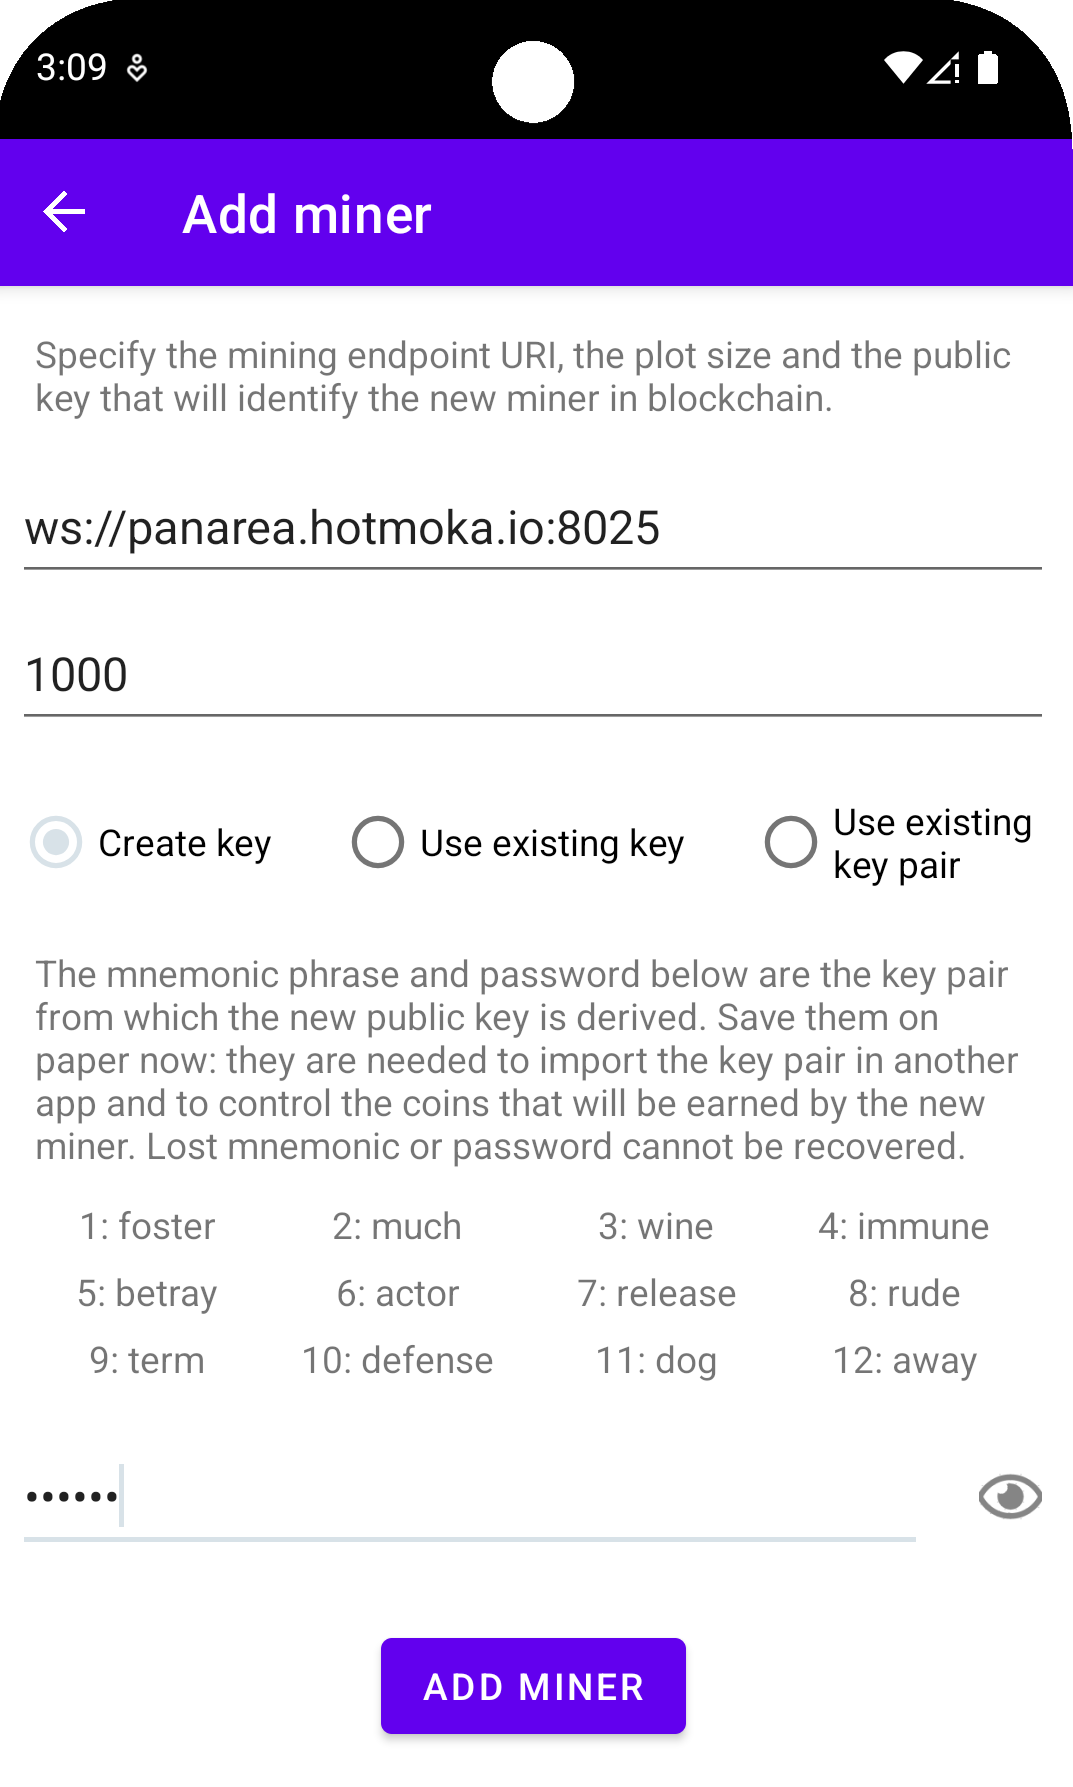
\includegraphics[width=\textwidth/3]{pictures/mokaminter_add_miner}
%  \end{center}
%  \caption{Specification of the parameters for the creation of a miner.}
%  \label{fig:mokaminter_add_miner}
%\end{figure}

%\begin{figure}[b]
%  \begin{center}
%    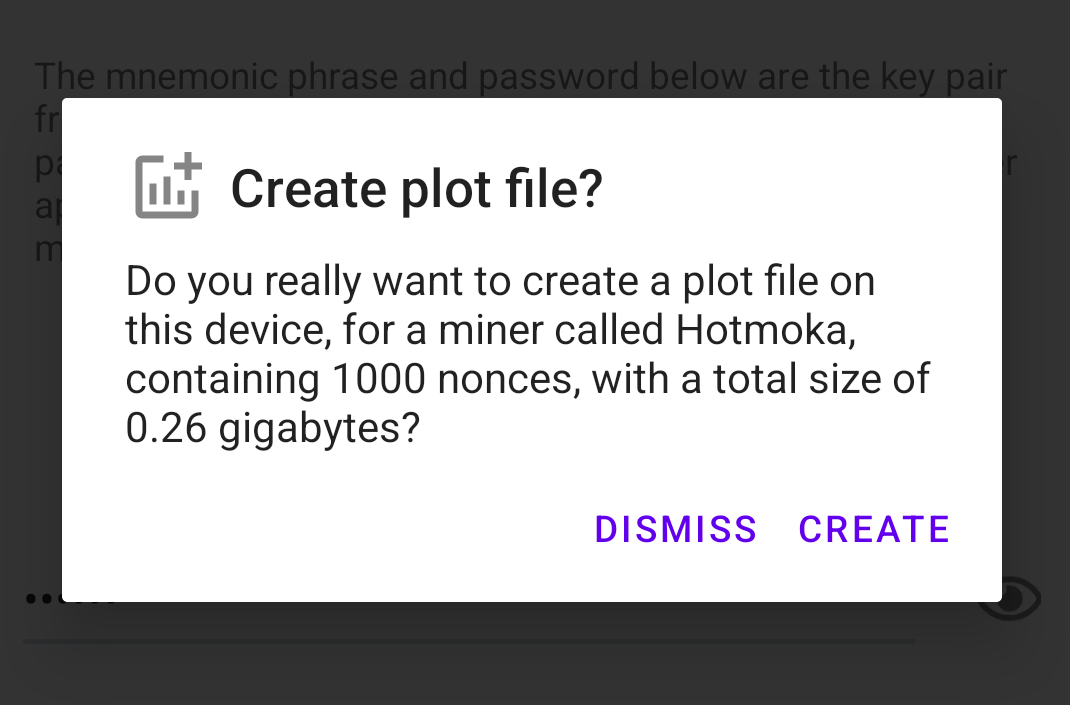
\includegraphics[width=\textwidth/3]{pictures/mokaminter_confirmation}
%  \end{center}
%  \caption{Confirmation is required before creating a new plot file.}
%  \label{fig:mokaminter_confirmation}
%\end{figure}

%\begin{figure}[t]
%  \begin{center}
%    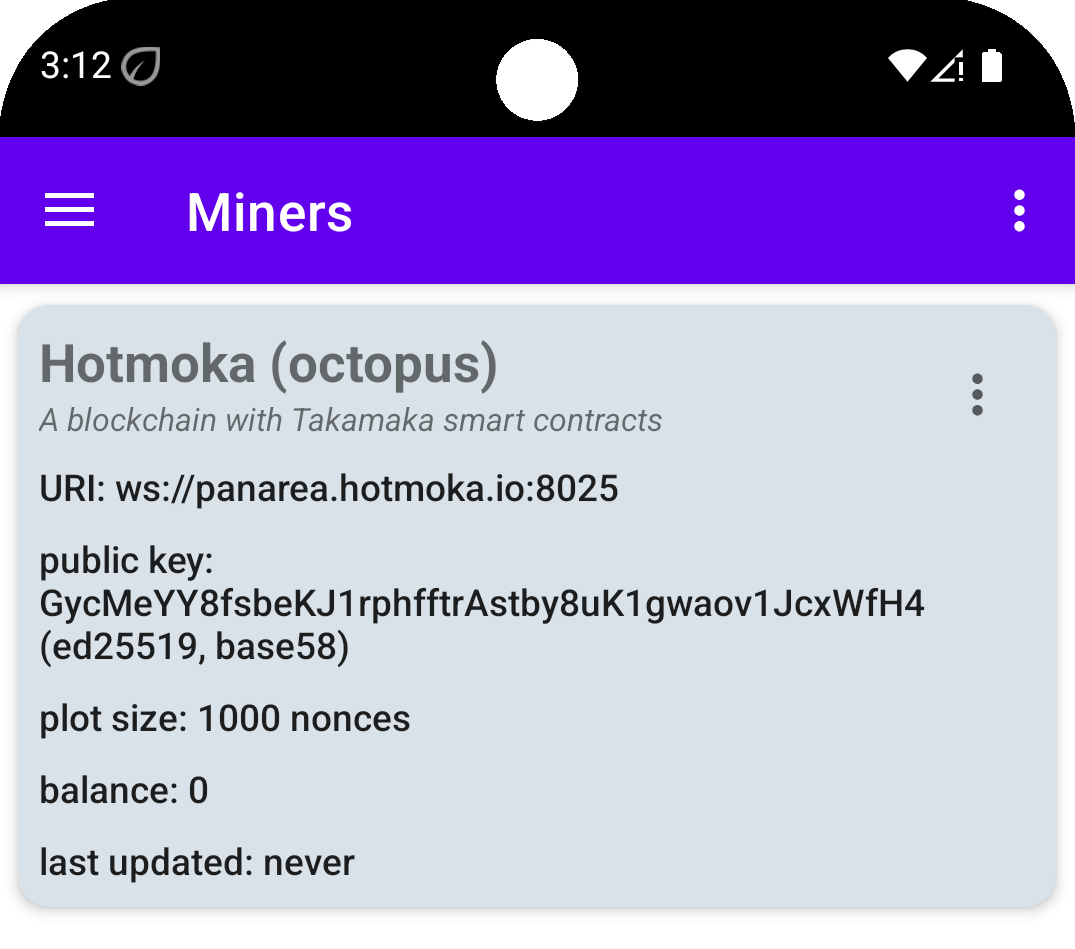
\includegraphics[width=\textwidth/3]{pictures/mokaminter_mining}
%  \end{center}
%  \caption{A new tile for a miner, working in the background. Eventually, its
%  cryptocurrency balance will increase.}
%  \label{fig:mokaminter_mining}
%\end{figure}

\vspace{0.5ex}\noindent\textbf{Security considerations.}
%
A lost or stolen device is a relatively frequent event.
If private keys were kept in the device, who finds
or steals the device could also steal the cryptocurrency accumulated while mining with such keys.
Therefore, Mokaminter does not store private keys.
Namely, only the public key is needed to create the plot (Def.~\ref{def:nonce_construction}), and
the app can forget the private key. This entails, however,
that the user must not lose the $12$ words of the key pair,
or otherwise the earned crypto becomes inaccessible.
The use of the miner's \emph{public} key for the construction of its nonces
(step.~\ref{step:nonce_construction:seed}
of Def.~\ref{def:nonce_construction}) might seem
to be a security issue, since anyone can impersonate a miner.
But that impersonation could only be a help for the impersonated miner:
the impersonator might create nonces that are so good to win
the mining competition, whose reward will go to the public key (hence to the miner);
or nonces that lose the mining competition, in which case they are just ignored;
or syntactically illegal nonces, in which case Mokamint bans the IP of the impersonator
(it does not ban the public key of the miner). In any case, the impersonated miner
can only win from the impersonation.

\vspace{0.5ex}\noindent\textbf{Usability considerations.}
%
A mobile app has quite different usability considerations than a desktop application.
A first one is about feedback.
A desktop user can check warnings, error messages and logs.
In a mobile app, this is possible
but uncomfortable for most users. Therefore, Mokaminter gives feedback through
a heartbeat effect at each challenge, to inform the user that it is
actually mining. Moreover, network disconnection
turns the miner's tile gray in the list of miners.
%
Another usability issue is related to the insertion of the
$12$ words, to import an existing key pair.
This is frustrating and error-prone with the software keyboard of a mobile device.
Thus, Mokaminter autocompletes words while typing.
%
A last issue is the risk of specifying a plot dimension that is
too large to complete the plot's creation in a reasonable time:
this would hang the device and drain its battery. To avoid this risk,
Mokaminter imposes a maximum plot dimension, that the user can override
with an explicit decision.

\vspace{0.5ex}\noindent\textbf{Technical considerations.}
%
Mokaminter uses websockets for network connections,
that perfectly match the continuous, bidirectional flow of challenges
and answers (Fig.~\ref{fig:mining}). But network connection in a
mobile device may be relatively unstable (thick walls, tunnels, network switches).
Mokaminter tries to reconnect if the connection is lost or
if it has not received any challenge for some time. If reconnection fails, it
tries again after a minute, to avoid draining the battery with too
frequent attempts. Background mining execution and battery optimization
are a complication solved through the official
Android good practice~\cite{background-tasks}
that ensures a background task to run continously,
leveraging either a \texttt{WorkManager} or a \texttt{JobService}, depending on the
Android version, together with a foreground notification.
%
%Another technical issue is related to the background task for mining.
%The Android system is extremely restrictive with background
%tasks, since they might drain the battery. There are official guidelines
%for them, but they changed across different Android versions and
%phone manufacturers often add extra constraints. Many phones
%turn Mokaminter off overnight, when
%the Android system enters a special \emph{doze mode}. If this happens, it is enough
%for the user
%to turn it on again in the morning. A better solution does not seem in sight, at the moment.


\section{Experiments}\label{sec:experiments}

This section reports experiments with the plotting and mining phases.
We selected a mobile phone, a tablet and a desktop computer, all relatively old devices
with quite limited resources. The mobile phone and
the tablet ran the Mokaminter miner, while the desktop computer ran a desktop miner and it has been
chosen to compare the results of the mobile devices with those of a home
computer with a stable internet connection.

Fig.~\ref{fig:plotting_phase_experiments} reports results about the plotting phase.
It confirms that this phase is expensive, as required, with a cost that grows linearly with the
plot size, as expected since a plot is a linear collection of nonces
(Fig.~\ref{fig:waiting_time}). Of course, a faster CPU, such as that of the desktop computer,
builds the plot in a shorter time.

\begin{figure}[t]
  \begin{center}
    \begin{tabular}{|c|c||c|c|c|}
      \hline
      \textbf{device} & \textbf{type} & \textbf{nonces} & \textbf{size} & \textbf{time} \\\hline\hline
      Xiami 11 Lite 5G NE & phone & 1000 & 0.26GB & 1m13s \\\hline
      Xiami 11 Lite 5G NE & phone & 5000 & 1.28GB & 6m03s \\\hline
      Xiami 11 Lite 5G NE & phone & 10000 & 2.56GB & 12m05s \\\hline\hline
      Samsung Galaxy Tab S6 Lite & tablet & 1000 & 0.26GB & 2m15s \\\hline
      Samsung Galaxy Tab S6 Lite & tablet & 5000 & 1.28GB & 11m12s \\\hline
      Samsung Galaxy Tab S6 Lite & tablet & 10000 & 2.56GB & 22m21s \\\hline\hline
      Intel NUC8i5BEH & desktop & 1000 & 0.26GB & 20s \\\hline
      Intel NUC8i5BEH & desktop & 5000 & 1.28GB & 1m40s \\\hline
      Intel NUC8i5BEH & desktop & 10000 & 2.56GB & 3m24s \\\hline
    \end{tabular}
  \end{center}
  \caption{Results about the plotting phase. \emph{Type} is the type of device;
    \emph{nonces} is the number of nonces in the plot file;
    \emph{size} is the size of the plot file; \emph{time} is the time for creating the
    plot file (Def.~\ref{def:nonce_construction}, repeated for each nonce in the plot).
    Data has been collected by manually creating the plots.
  }
  \label{fig:plotting_phase_experiments}
\end{figure}

Fig.~\ref{fig:mining_phase_experiments} reports results about the mining phase.
It shows that CPU and RAM costs of Mokaminter are minimal, as well as its
amount of data exchanged through the network. It shows that answering challenges is quick (as required).
Finally, it shows that a mobile miner in a phone or tablet, surely experiencing some network swaps
and disconnections, yields similar mining earnings to those
of a desktop computer using a reliable home internet connection. Note that we cannot express
the earnings in fiat currency, since Hotmoka's mokas are not currently exchangeable.

\begin{figure}[t]
  \begin{center}
    \begin{tabular}{|c|c||c|c|c|c|c|}
      \hline
      \textbf{device} & \textbf{type} & \textbf{CPU} & \textbf{RAM} & \textbf{network} & \textbf{per chall.} & \textbf{earned crypto} \\\hline\hline
      Xiami 11 Lite 5G NE & phone & 0.56\% & 2.4\% (192MB) & 3.36MB & 0.207s & 373.30 mokas \\\hline
      Samsung Galaxy Tab S6 Lite & tablet & 0.23\% & 3.5\% (140MB) & 3.38MB & 0.225s & 266.63 mokas \\\hline
      Intel NUC8i5BEH & desktop & 0.09\% & 1.4\% (224MB) & 3.39MB & 0.019s & 319.95 mokas \\\hline
    \end{tabular}
  \end{center}
  \caption{Results about the mining phase for the mainnet of the Hotmoka blockchain.
    \emph{Type} is the type of device; \emph{CPU} is the
    percent of the CPU power of the device used for mining;
    \emph{RAM} is the percent (and absolute value) of the
    RAM of the device used for mining; \emph{network} is the amount of data exchanged during one day of mining;
    \emph{per chall.} is the average time, in seconds, for answering each challenge
    (steps~\ref{step:deadline_mining:minimize}
    and~\ref{step:deadline_mining:compute_deadline} of Alg.~\ref{alg:deadline_mining});
    \emph{earned crypto} is the amount of crypto
    earned during one day of mining (\emph{moka} is the crypto unit of Hotmoka). Data has been collected
    through logs and the \texttt{top} Linux utility, run in the device through the Android Device Bridge
    (\texttt{adb}). Network usage has been collected through the app management page of Android and
    the \texttt{vnstat} Linux utility.
  }
  \label{fig:mining_phase_experiments}
\end{figure}

These mining experiments have been performed against the mainnet of Hotmoka, that creates a block every $20$ seconds
on average. Therefore, column \textbf{per chall.} of Fig.~\ref{fig:mining_phase_experiments} is actually telling us that
Mokaminter sits idle for around $99\%$ of its time, waiting at step~\ref{step:deadline_mining:wait}
of Alg.~\ref{alg:deadline_mining}. Together with the very limited CPU and RAM costs
(Fig.~\ref{fig:mining_phase_experiments}), it suggests that Mokaminter's battery use should be minimal.
An exact evaluation is difficult since it highly depends on the other apps
installed in the device and on the usage pattern of the device by its user.
In order to get some hint, in realistic conditions, we have installed Mokaminter on the personal phone of
a group of $11$ professors and students from the UFMA university in Brazil
(other potential users owned only an iPhone and could not take part in the experiment).
Each of them created a miner for the Hotmoka blockchain
and let it run in the phone for a day. At the end, they consulted the
settings page for Mokaminter in Android and reported the
percent of battery used.
The result is that Mokaminter consumed only $0.27\%$ of battery power, on average.
The quality of mobile internet in the area of Brazil where
the experiment has been conducted is low in comparison to other areas
of the country. Still, Mokaminter worked and mined correctly.
To push this test to the limit, Mokaminter has also been used during
an international flight, with the minimal free internet connection
on board. Even in this adverse condition, it worked and mined without problems.

%In conclusion, these simple, yet limited experiments show that
%Mokaminter is actually working, in various internet conditions,
%and that its comsumption is minimal, in terms of bandwidth and
%battery usage.

%Telefono: chiave GD9cM3Jh6t7gMjPL4nTg5CHyZNyV8fKLuumP41GUrd44
%746601836927020031549974
%Tablet: chiave 9d8nD1BzsdKqGd87KbjTuU9G1DNbKsfztoxJMJU8yGSw
%533263217568183966578848
%Desktop: chiave 2hrKnNit4p8YxffZNFvn5KdC6Wj8xnTGRVb69W2yihfp
%639913715574334030959134

\section{Conclusion}\label{sec:conclusion}

This paper advocates mining in a mobile device, for blockchains based on
proof of space. It describes our Mokaminter
mining app for Android, showing its minimal
CPU, RAM, data exchange and battery costs, which is important in a mobile device.
Therefore, mobile mining is actually feasible.
Mokaminter is meant for blockchains based on the Mokamint engine~\cite{mokamint-source-code} and
the proof of space algorithm in~\cite{Spoto25}, but we think
that it could be adapted to other blockchains based on
proof of space, such as Chia~\cite{AbusalahACKPR17}.

If a proof of space blockchain reaches success, the pressure to use larger disk space
for mining would likely rule out mining on mobile devices.
But a mobile mining app remains a precious tool to start new blockchains
and lead them to the success that then makes such an app outdated.



\bibliography{biblio}

\end{document}
